In this chapter, we analyze the fourth experiment group, that is, the impact of having different amounts of clients, per scoring technique, in a Blockchain-based Federated Learning system. In this set of experiments, all properties of the system are static, except for the amount of clients, which varies between 5, 10, 25 and 50, per each scoring mechanism.

\todo{}

\section{Execution Time, Transaction Cost and Latency}

The results regarding execution time and transaction cost and latency can be visualized in \autoref{fig:clients_time}. As can be seen in the picture, all scoring algorithms present different growths regarding execution time with the increase of training clients.

One one hand, no scoring mechanism and Multi-KRUM present a quasi-linear execution time and mean round time growth. In Multi-KRUM, as previously discussed, the scores are calculated by the servers. Since the number of servers is independent of the number of clients, and is static, the growth is expected to be linear. On the other hand, BlockFlow and Marginal Gain present super-linear growths. Since the clients are the scorers and the clients increase, and each client has to score each other client, it is expected that the growth would be higher than with the remaining techniques.

% Tx latency is around the same, no matter how many devices we have. Ethereum has a relatively fixed capacity of transactions.

\begin{figure}[!hb]
    \centering
    \begin{subfigure}[b]{0.49\textwidth}
        \centering
        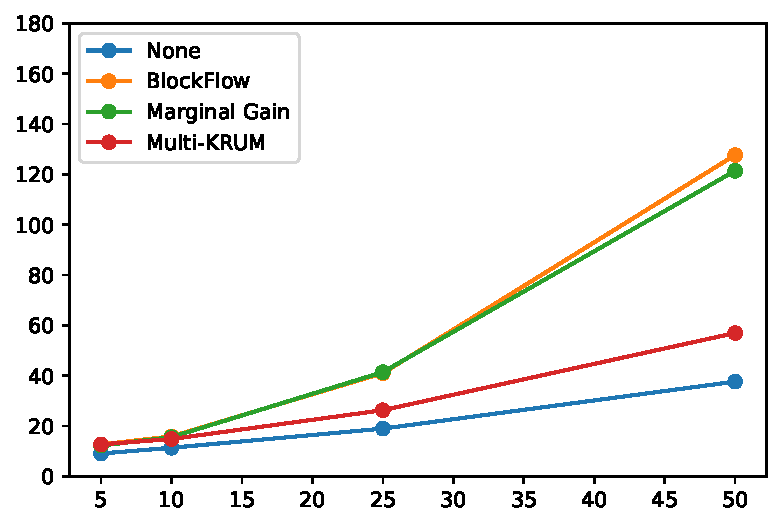
\includegraphics[width=\textwidth]{graphics/clients/e2e.pdf}
        \caption{E2E Time}
    \end{subfigure}
    \hfill
    \begin{subfigure}[b]{0.49\textwidth}
        \centering
        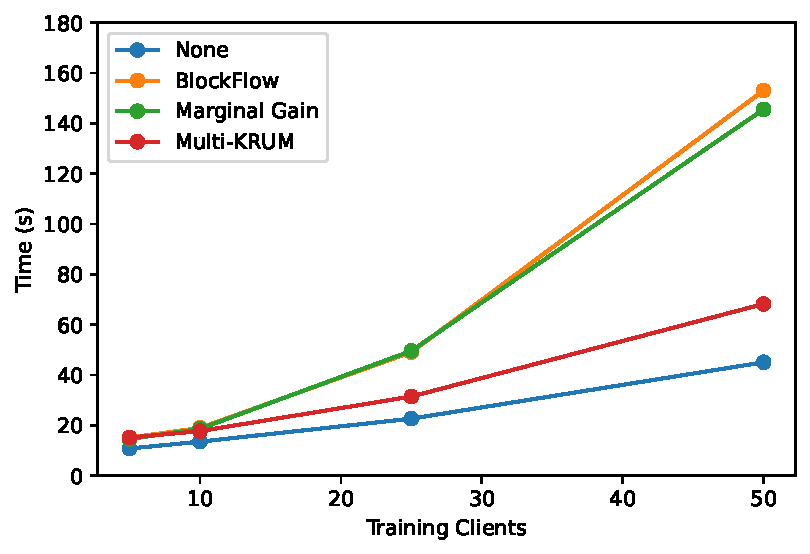
\includegraphics[width=\textwidth]{graphics/clients/round.pdf}
        \caption{Mean Round Time}
    \end{subfigure}
    \caption{Time Metrics Per Training Clients}
    \label{fig:clients_time}
\end{figure}

\begin{figure}[!hb]
    \centering
    \begin{subfigure}[b]{0.49\textwidth}
        \centering
        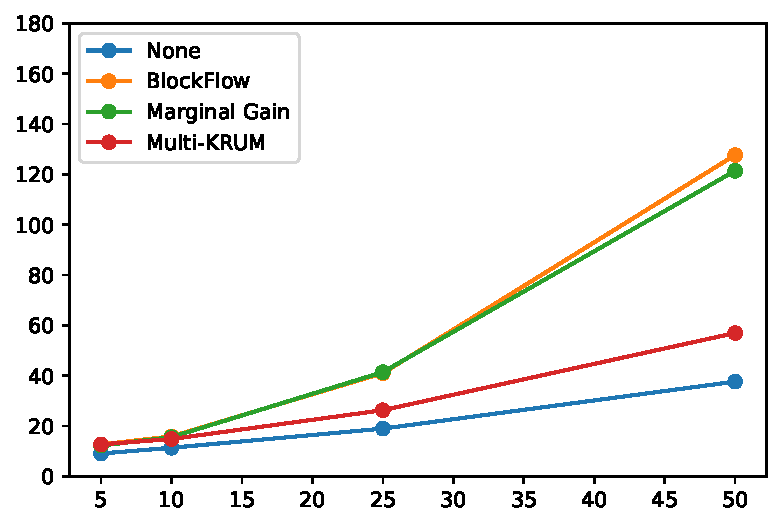
\includegraphics[width=\textwidth]{graphics/clients/e2e.pdf}
        \caption{E2E Time}
    \end{subfigure}
    \hfill
    \begin{subfigure}[b]{0.49\textwidth}
        \centering
        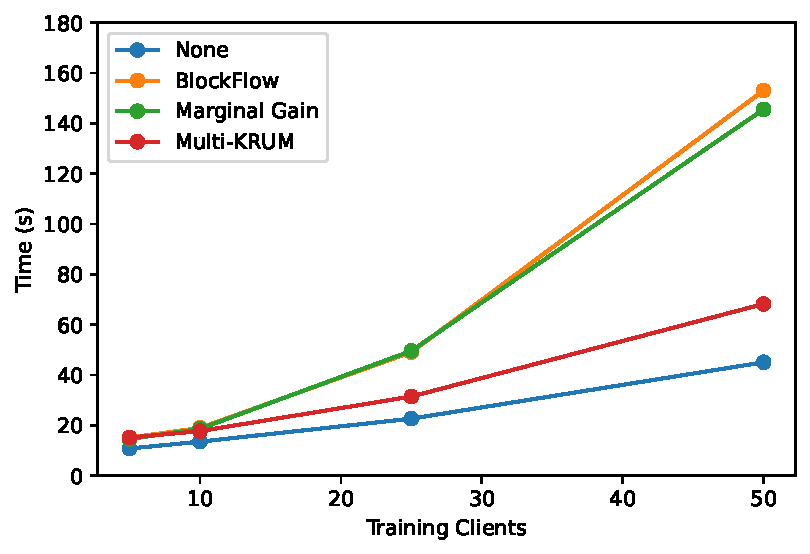
\includegraphics[width=\textwidth]{graphics/clients/round.pdf}
        \caption{Mean Round Time}
    \end{subfigure}
    \hfill
    \begin{subfigure}[b]{0.49\textwidth}
        \centering
        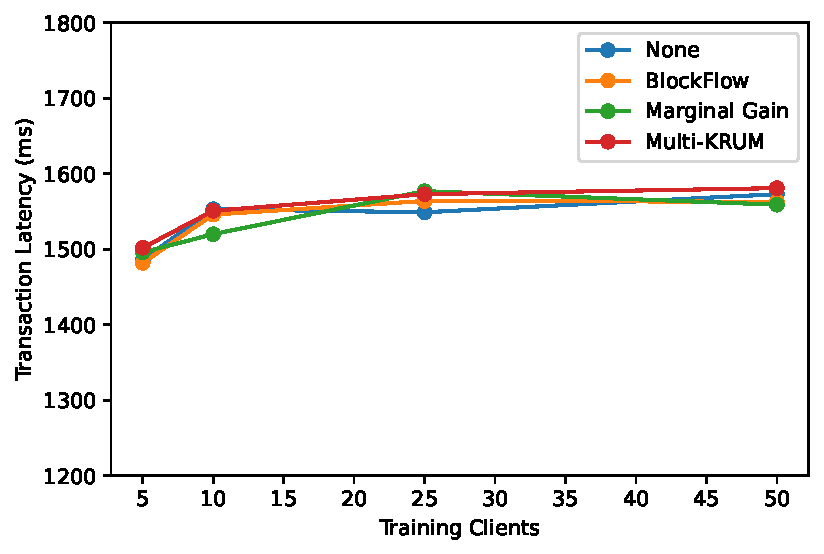
\includegraphics[width=\textwidth]{graphics/clients/tx_latency.pdf}
        \caption{Transaction Latency}
    \end{subfigure}
    \hfill
    \begin{subfigure}[b]{0.49\textwidth}
        \centering
        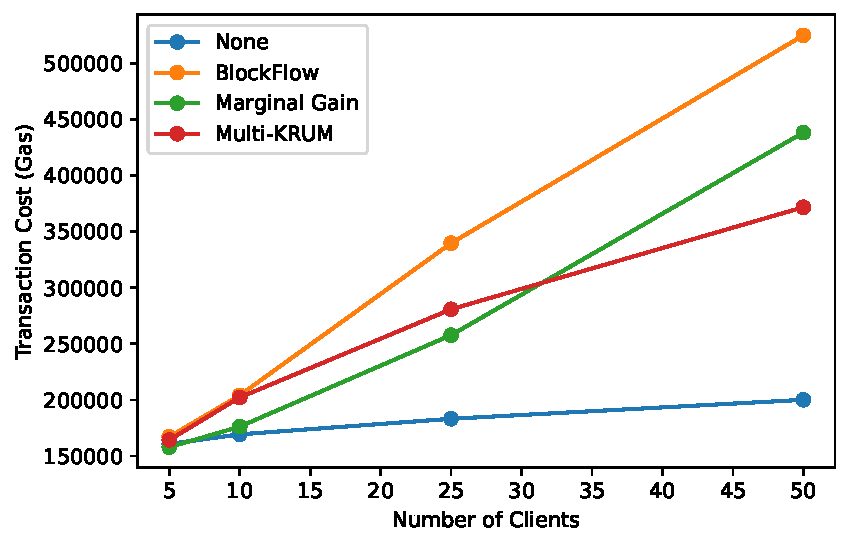
\includegraphics[width=\textwidth]{graphics/clients/tx_cost.pdf}
        \caption{Transaction Cost}
    \end{subfigure}
    \caption{Time and Transaction Metrics Per Training Clients}
    \label{fig:clients_metrics}
\end{figure}

\section{Accuracy and Convergence}

\begin{figure}[!ht]
    \centering
    \begin{subfigure}[b]{0.49\textwidth}
        \centering
        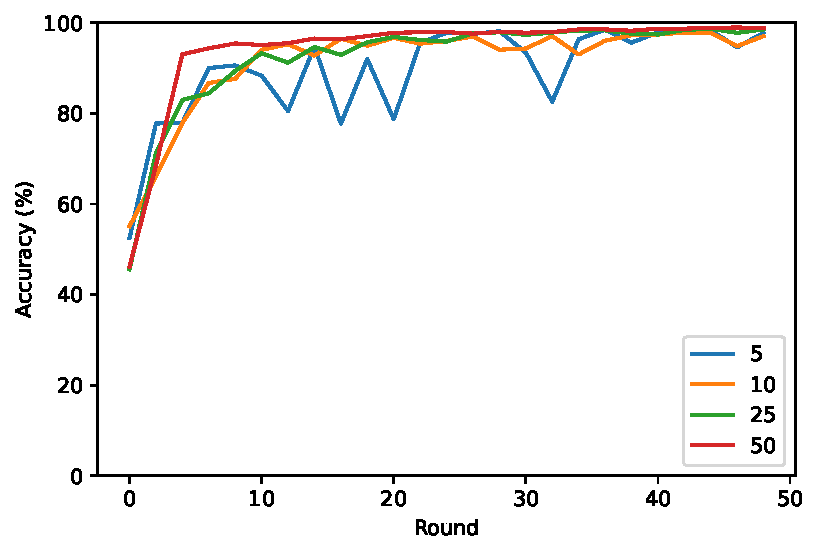
\includegraphics[width=\textwidth]{graphics/clients/accuracy_none.pdf}
        \caption{None}
    \end{subfigure}
    \hfill
    \begin{subfigure}[b]{0.49\textwidth}
        \centering
        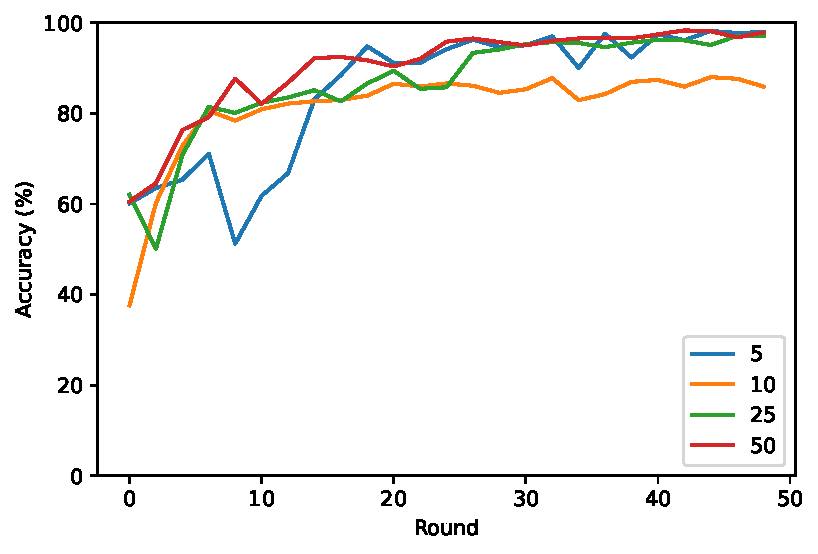
\includegraphics[width=\textwidth]{graphics/clients/accuracy_blockflow.pdf}
        \caption{BlockFlow}
    \end{subfigure}
    \hfill
    \begin{subfigure}[b]{0.49\textwidth}
        \centering
        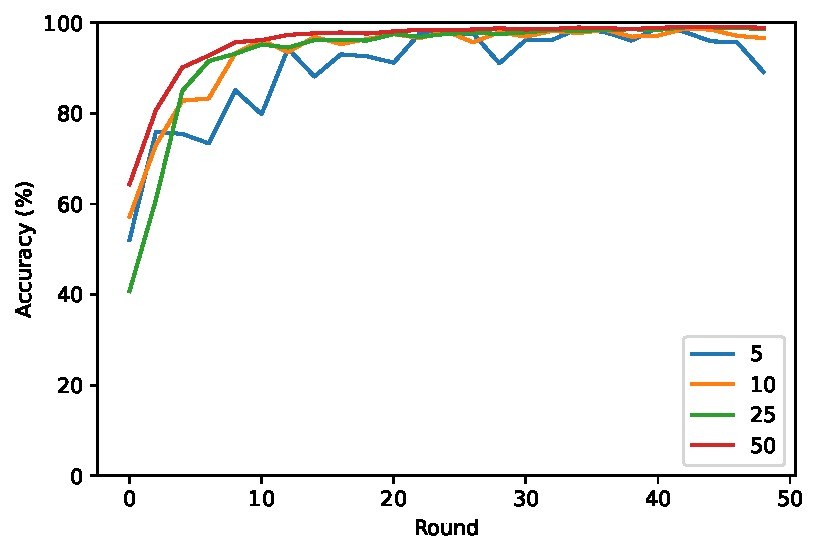
\includegraphics[width=\textwidth]{graphics/clients/accuracy_marginalgain.pdf}
        \caption{Marginal Gain}
    \end{subfigure}
    \hfill
    \begin{subfigure}[b]{0.49\textwidth}
        \centering
        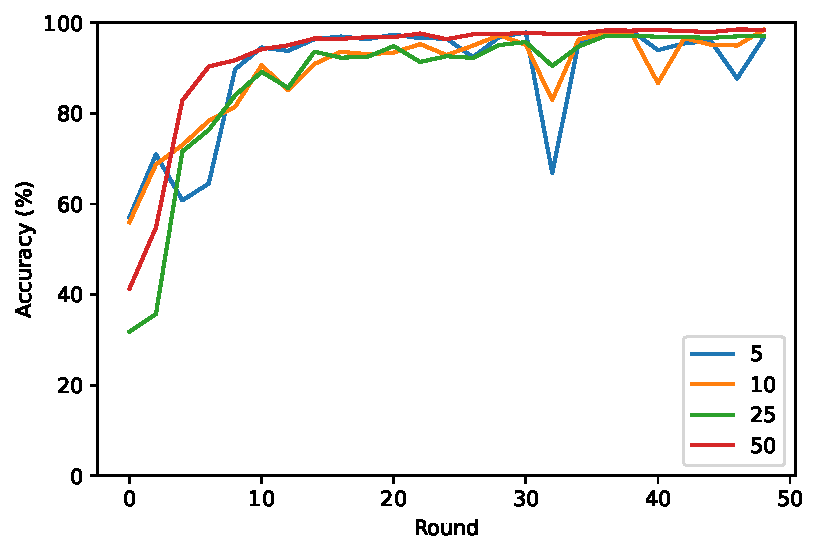
\includegraphics[width=\textwidth]{graphics/clients/accuracy_multikrum.pdf}
        \caption{Multi-KRUM}
    \end{subfigure}
    \caption{Accuracy Per Training Clients}
    \label{fig:clients_accuracy}
\end{figure}


\section{Communication Costs}


\section{Computation Costs}


\section{Conclusions} % and improvements? and limitations?

\clearpage

\begin{figure}[!hp]
    \centering
    \begin{subfigure}[b]{0.49\textwidth}
        \centering
        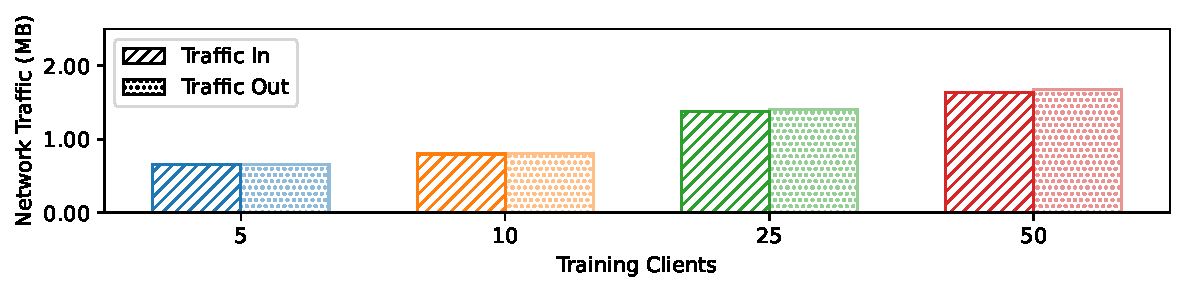
\includegraphics[width=\textwidth]{graphics/clients/net_none_client.pdf}
        \caption{None}
    \end{subfigure}
    \hfill
    \begin{subfigure}[b]{0.49\textwidth}
        \centering
        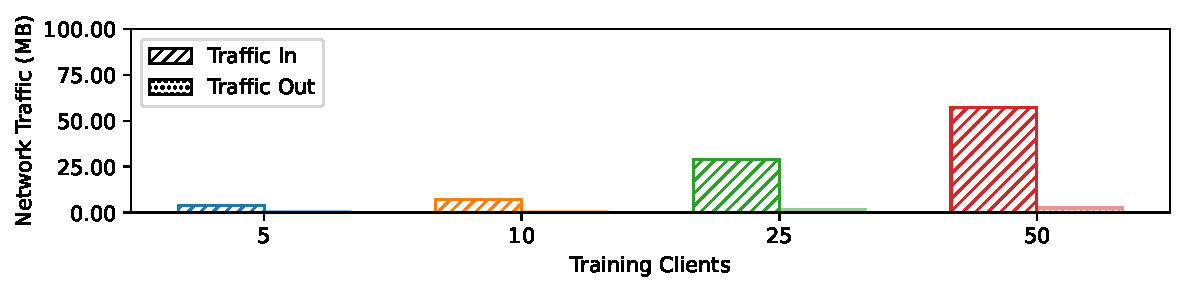
\includegraphics[width=\textwidth]{graphics/clients/net_blockflow_client.pdf}
        \caption{BlockFlow}
    \end{subfigure}
    \hfill
    \begin{subfigure}[b]{0.49\textwidth}
        \centering
        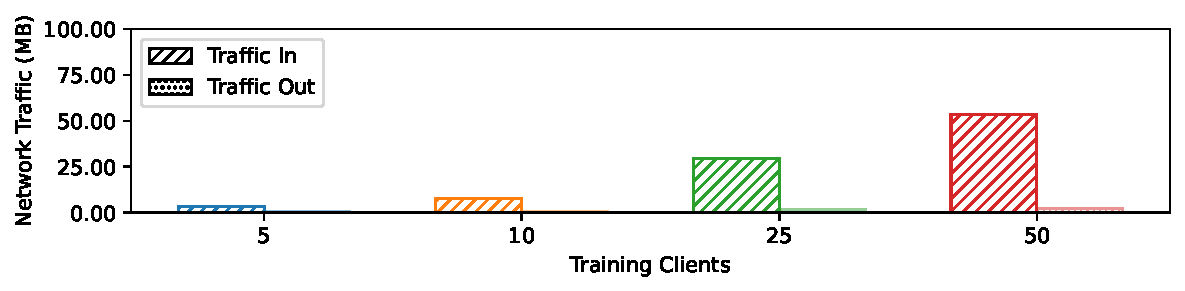
\includegraphics[width=\textwidth]{graphics/clients/net_marginalgain_client.pdf}
        \caption{Marginal Gain}
    \end{subfigure}
    \hfill
    \begin{subfigure}[b]{0.49\textwidth}
        \centering
        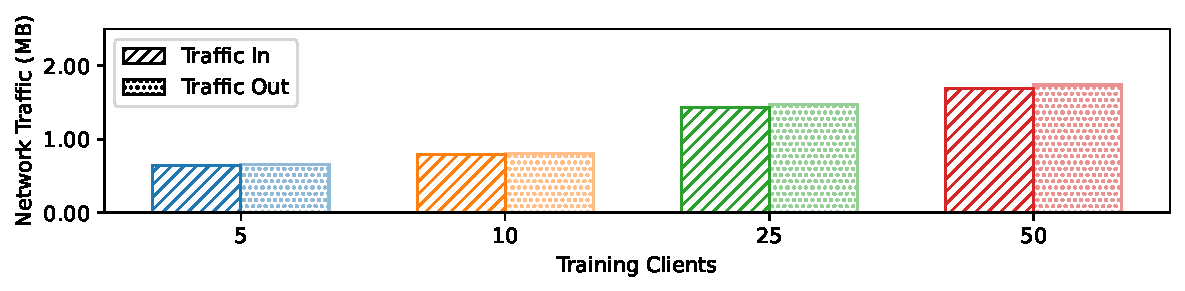
\includegraphics[width=\textwidth]{graphics/clients/net_multikrum_client.pdf}
        \caption{Multi-KRUM}
    \end{subfigure}
    \caption{Network Traffic on Training Clients Per Training Clients}
    \label{fig:net_clients_degree_clients}
\end{figure}

\begin{figure}[!hp]
    \centering
    \begin{subfigure}[b]{0.49\textwidth}
        \centering
        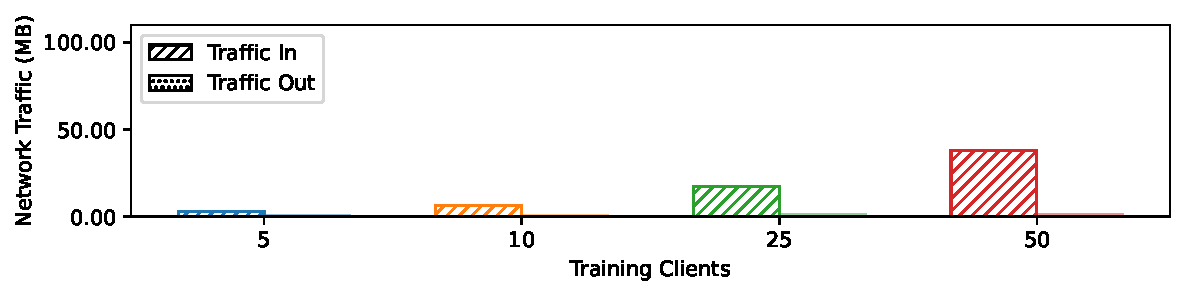
\includegraphics[width=\textwidth]{graphics/clients/net_none_server.pdf}
        \caption{None}
    \end{subfigure}
    \hfill
    \begin{subfigure}[b]{0.49\textwidth}
        \centering
        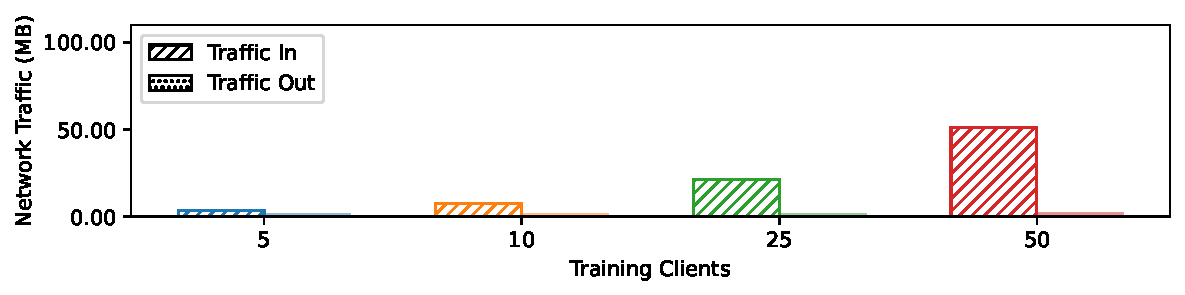
\includegraphics[width=\textwidth]{graphics/clients/net_blockflow_server.pdf}
        \caption{BlockFlow}
    \end{subfigure}
    \hfill
    \begin{subfigure}[b]{0.49\textwidth}
        \centering
        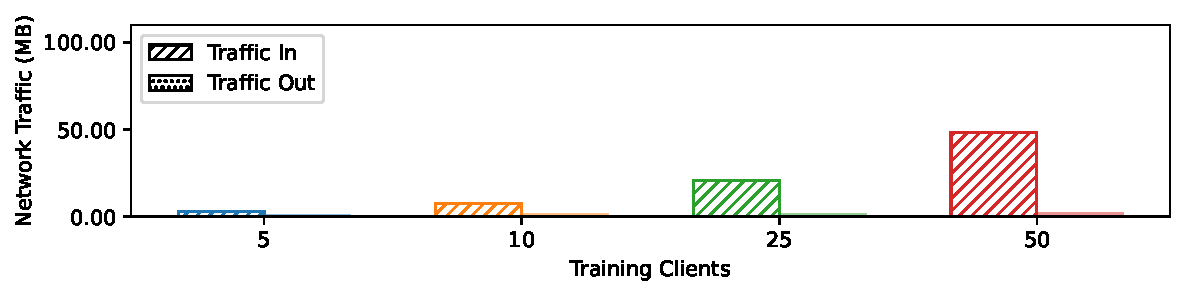
\includegraphics[width=\textwidth]{graphics/clients/net_marginalgain_server.pdf}
        \caption{Marginal Gain}
    \end{subfigure}
    \hfill
    \begin{subfigure}[b]{0.49\textwidth}
        \centering
        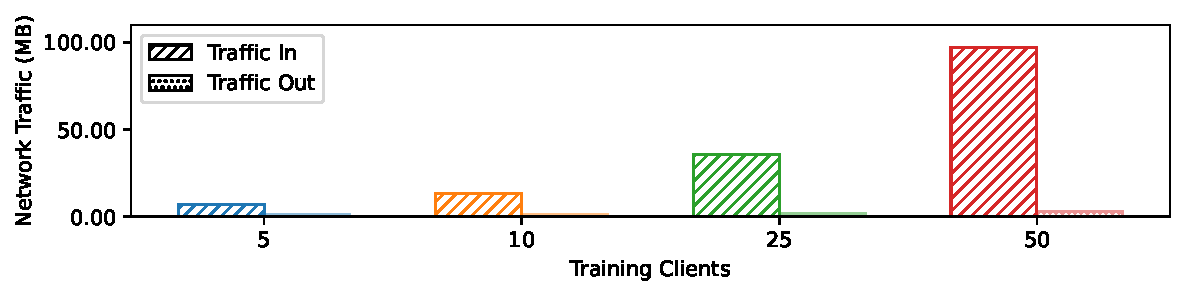
\includegraphics[width=\textwidth]{graphics/clients/net_multikrum_server.pdf}
        \caption{Multi-KRUM}
    \end{subfigure}
    \caption{Network Traffic on Computing Servers Per Training Clients}
    \label{fig:net_clients_degree_server}
\end{figure}

\begin{figure}[!hp]
    \centering
    \begin{subfigure}[b]{0.49\textwidth}
        \centering
        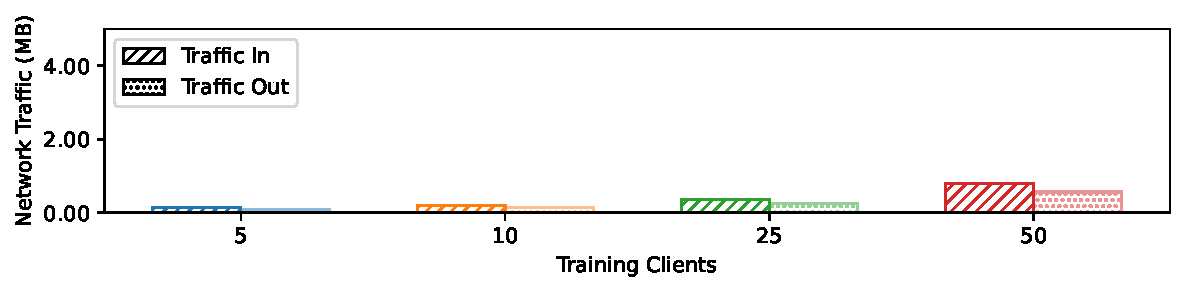
\includegraphics[width=\textwidth]{graphics/clients/net_none_miner.pdf}
        \caption{None}
    \end{subfigure}
    \hfill
    \begin{subfigure}[b]{0.49\textwidth}
        \centering
        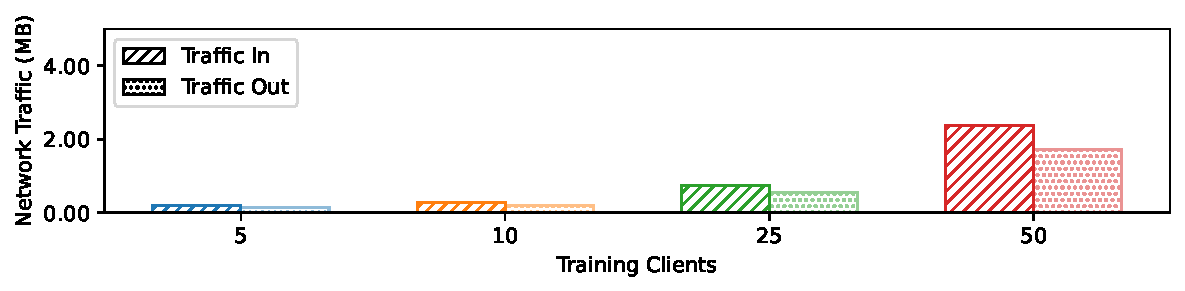
\includegraphics[width=\textwidth]{graphics/clients/net_blockflow_miner.pdf}
        \caption{BlockFlow}
    \end{subfigure}
    \hfill
    \begin{subfigure}[b]{0.49\textwidth}
        \centering
        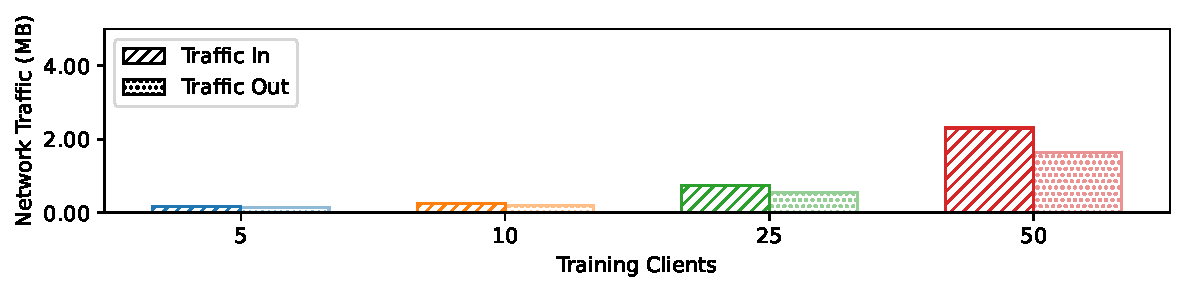
\includegraphics[width=\textwidth]{graphics/clients/net_marginalgain_miner.pdf}
        \caption{Marginal Gain}
    \end{subfigure}
    \hfill
    \begin{subfigure}[b]{0.49\textwidth}
        \centering
        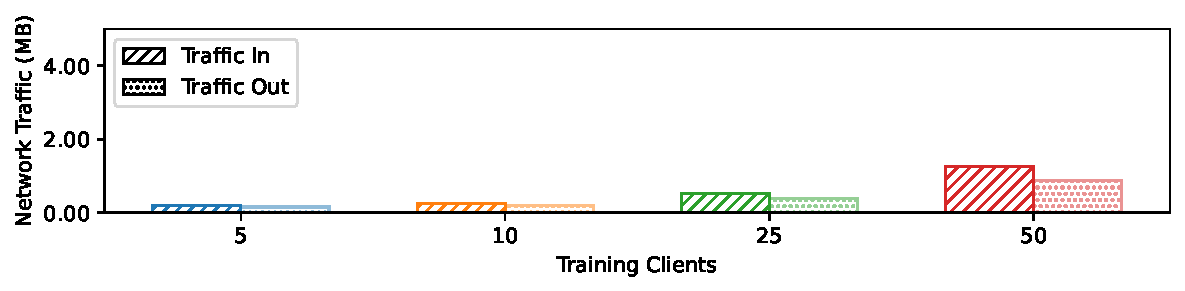
\includegraphics[width=\textwidth]{graphics/clients/net_multikrum_miner.pdf}
        \caption{Multi-KRUM}
    \end{subfigure}
    \caption{Network Traffic on Blockchain Nodes Per Training Clients}
    \label{fig:net_clients_degree_miner}
\end{figure}

\clearpage

\begin{figure}[!h]
    \centering
    \begin{subfigure}[b]{0.49\textwidth}
        \centering
        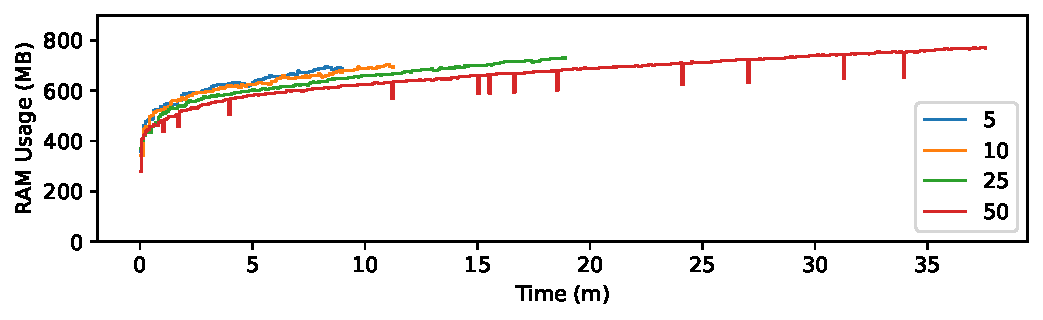
\includegraphics[width=\textwidth]{graphics/clients/ram_none_client.pdf}
        \caption{None}
    \end{subfigure}
    \hfill
    \begin{subfigure}[b]{0.49\textwidth}
        \centering
        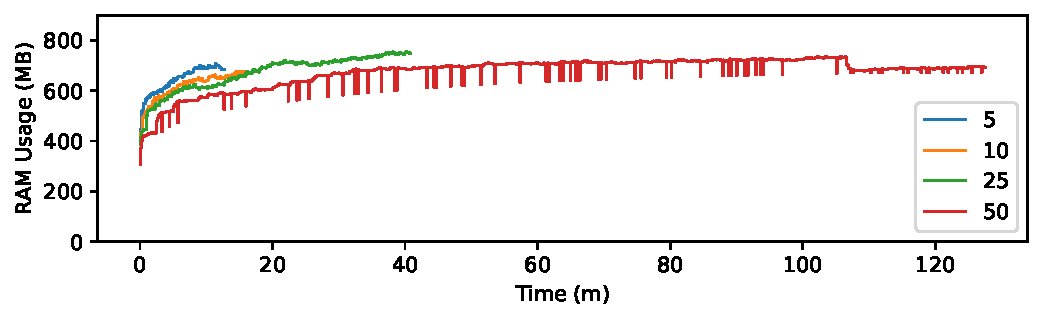
\includegraphics[width=\textwidth]{graphics/clients/ram_blockflow_client.pdf}
        \caption{BlockFlow}
    \end{subfigure}
    \hfill
    \begin{subfigure}[b]{0.49\textwidth}
        \centering
        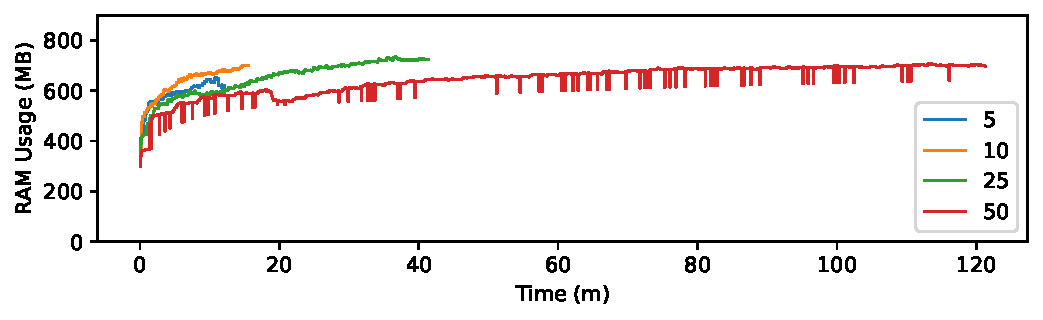
\includegraphics[width=\textwidth]{graphics/clients/ram_marginalgain_client.pdf}
        \caption{Marginal Gain}
    \end{subfigure}
    \hfill
    \begin{subfigure}[b]{0.49\textwidth}
        \centering
        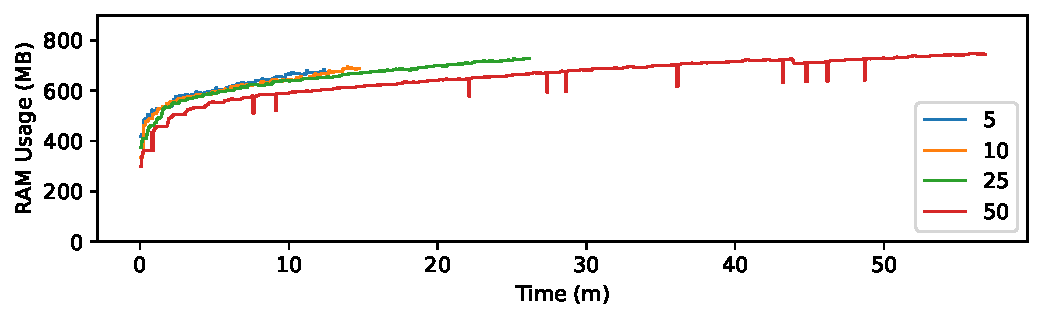
\includegraphics[width=\textwidth]{graphics/clients/ram_multikrum_client.pdf}
        \caption{Multi-KRUM}
    \end{subfigure}
    \caption{RAM Usage on Training Clients Per Training Clients}
    \label{fig:ram_clients_degree_clients}
\end{figure}

\begin{figure}[!h]
    \centering
    \begin{subfigure}[b]{0.49\textwidth}
        \centering
        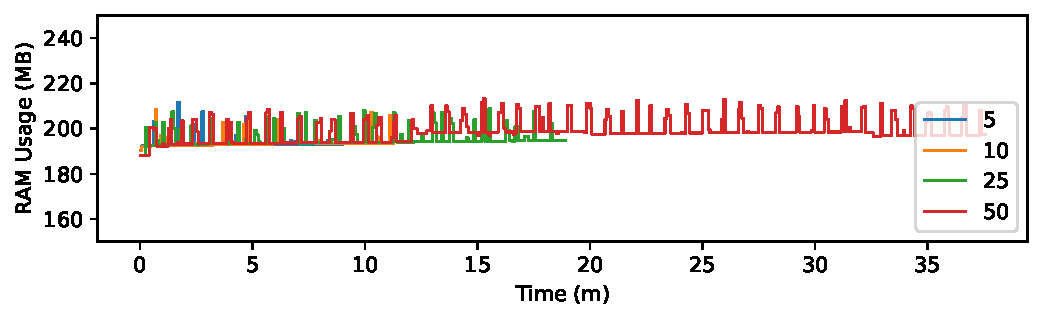
\includegraphics[width=\textwidth]{graphics/clients/ram_none_server.pdf}
        \caption{None}
    \end{subfigure}
    \hfill
    \begin{subfigure}[b]{0.49\textwidth}
        \centering
        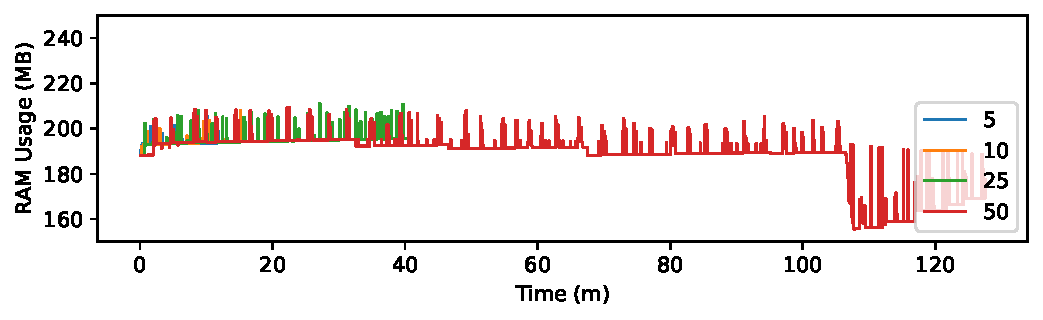
\includegraphics[width=\textwidth]{graphics/clients/ram_blockflow_server.pdf}
        \caption{BlockFlow}
    \end{subfigure}
    \hfill
    \begin{subfigure}[b]{0.49\textwidth}
        \centering
        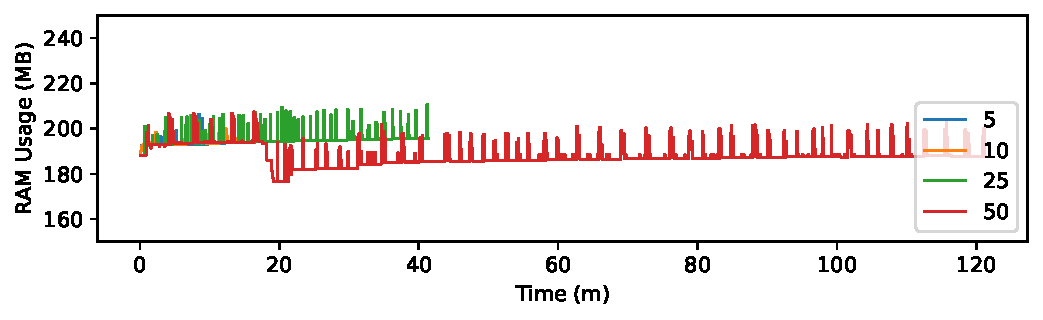
\includegraphics[width=\textwidth]{graphics/clients/ram_marginalgain_server.pdf}
        \caption{Marginal Gain}
    \end{subfigure}
    \hfill
    \begin{subfigure}[b]{0.49\textwidth}
        \centering
        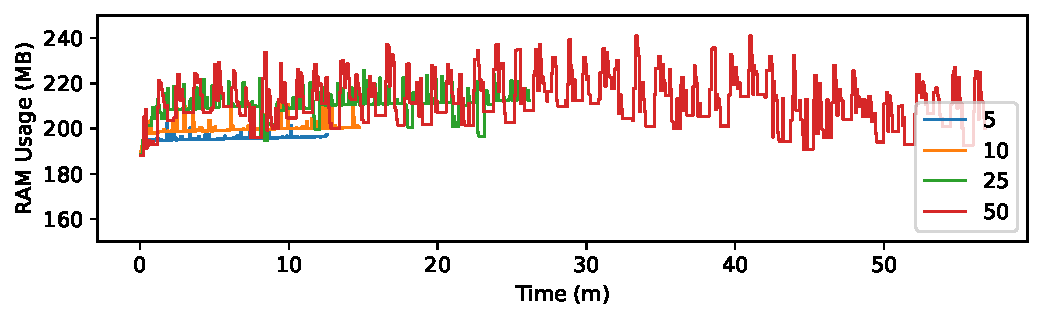
\includegraphics[width=\textwidth]{graphics/clients/ram_multikrum_server.pdf}
        \caption{Multi-KRUM}
    \end{subfigure}
    \caption{RAM Usage on Computing Servers Per Training Clients}
    \label{fig:ram_clients_degree_server}
\end{figure}

\begin{figure}[!h]
    \centering
    \begin{subfigure}[b]{0.49\textwidth}
        \centering
        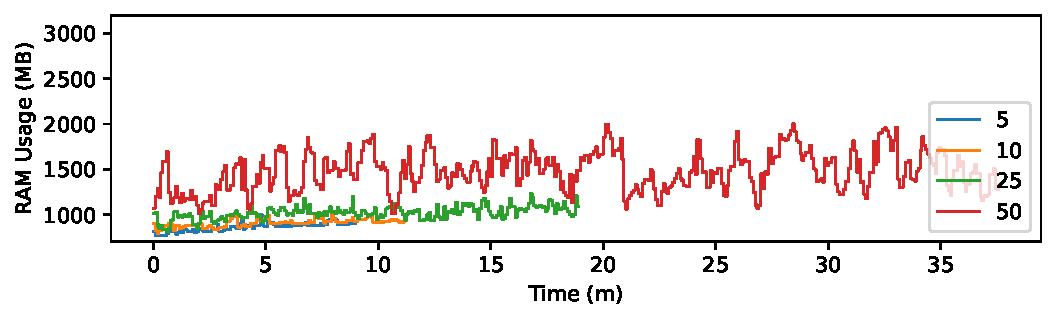
\includegraphics[width=\textwidth]{graphics/clients/ram_none_miner.pdf}
        \caption{None}
    \end{subfigure}
    \hfill
    \begin{subfigure}[b]{0.49\textwidth}
        \centering
        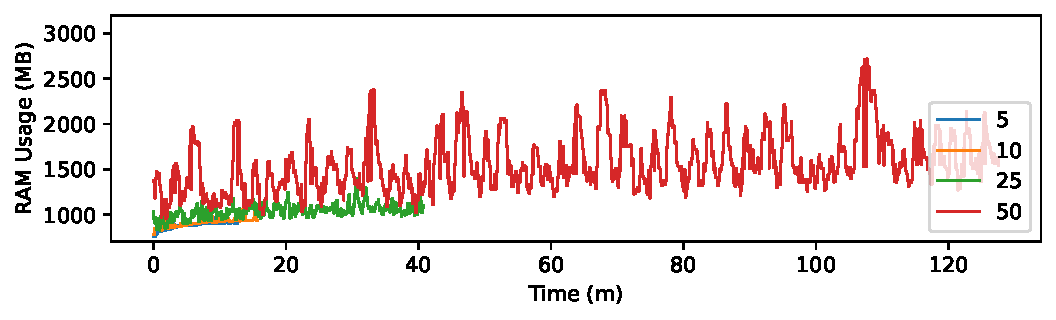
\includegraphics[width=\textwidth]{graphics/clients/ram_blockflow_miner.pdf}
        \caption{BlockFlow}
    \end{subfigure}
    \hfill
    \begin{subfigure}[b]{0.49\textwidth}
        \centering
        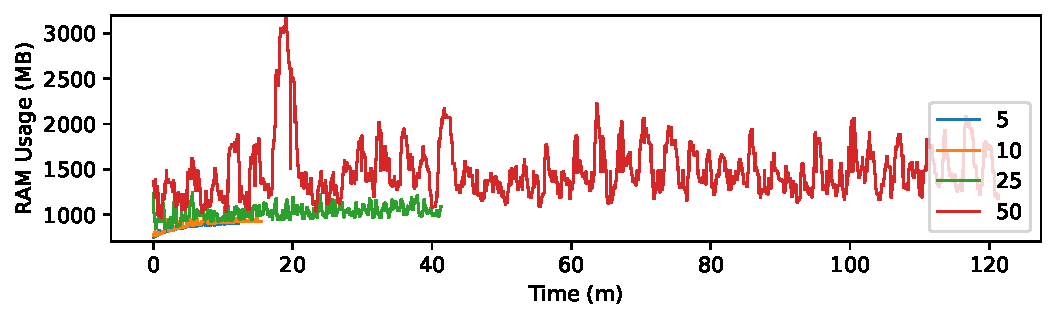
\includegraphics[width=\textwidth]{graphics/clients/ram_marginalgain_miner.pdf}
        \caption{Marginal Gain}
    \end{subfigure}
    \hfill
    \begin{subfigure}[b]{0.49\textwidth}
        \centering
        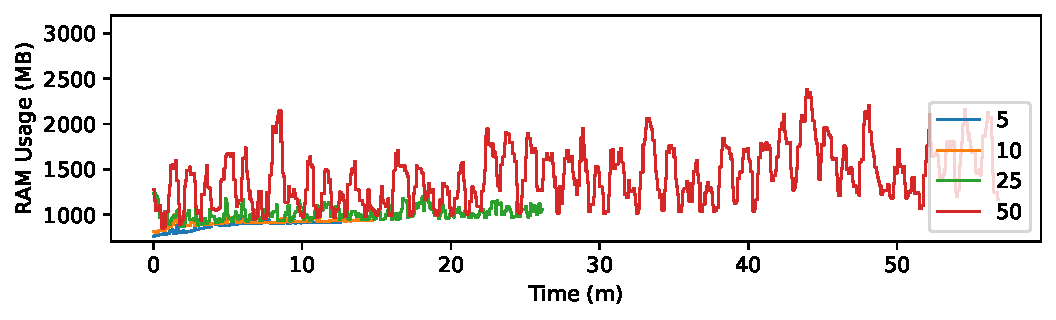
\includegraphics[width=\textwidth]{graphics/clients/ram_multikrum_miner.pdf}
        \caption{Multi-KRUM}
    \end{subfigure}
    \caption{RAM Usage on Blockchain Nodes Per Training Clients}
    \label{fig:ram_clients_degree_miner}
\end{figure}

\newpage

\begin{figure}[!h]
    \centering
    \begin{subfigure}[b]{0.49\textwidth}
        \centering
        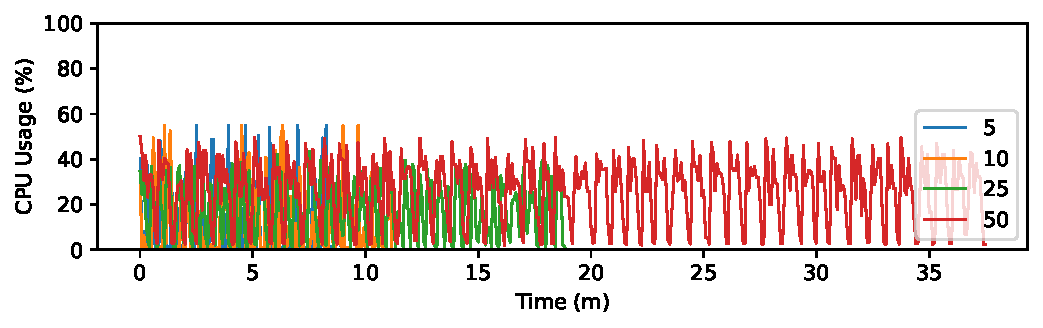
\includegraphics[width=\textwidth]{graphics/clients/cpu_none_client.pdf}
        \caption{None}
    \end{subfigure}
    \hfill
    \begin{subfigure}[b]{0.49\textwidth}
        \centering
        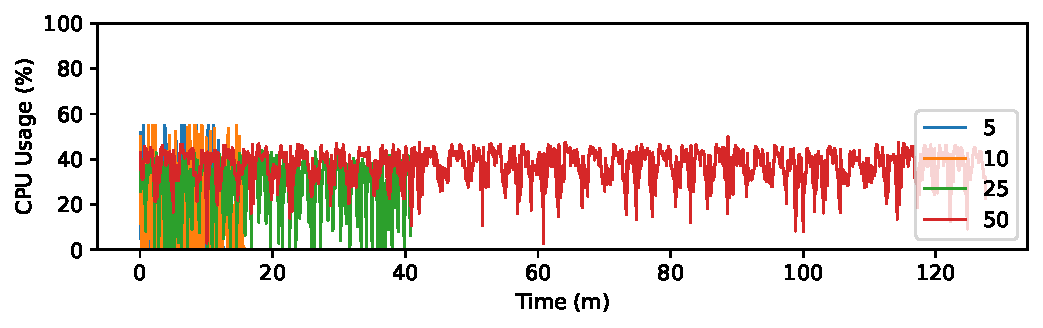
\includegraphics[width=\textwidth]{graphics/clients/cpu_blockflow_client.pdf}
        \caption{BlockFlow}
    \end{subfigure}
    \hfill
    \begin{subfigure}[b]{0.49\textwidth}
        \centering
        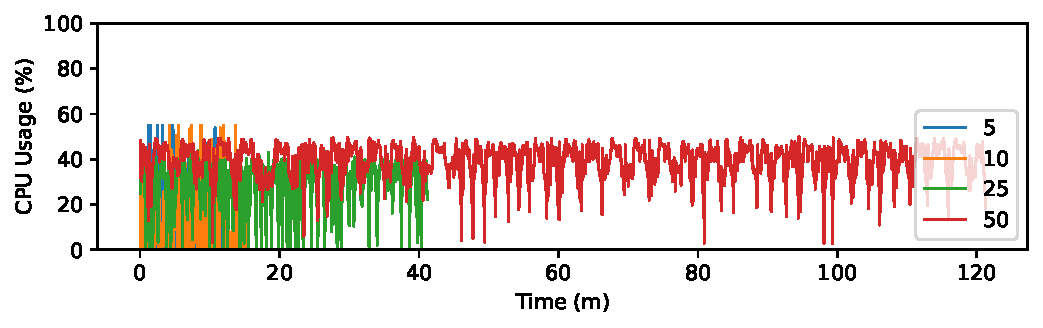
\includegraphics[width=\textwidth]{graphics/clients/cpu_marginalgain_client.pdf}
        \caption{Marginal Gain}
    \end{subfigure}
    \hfill
    \begin{subfigure}[b]{0.49\textwidth}
        \centering
        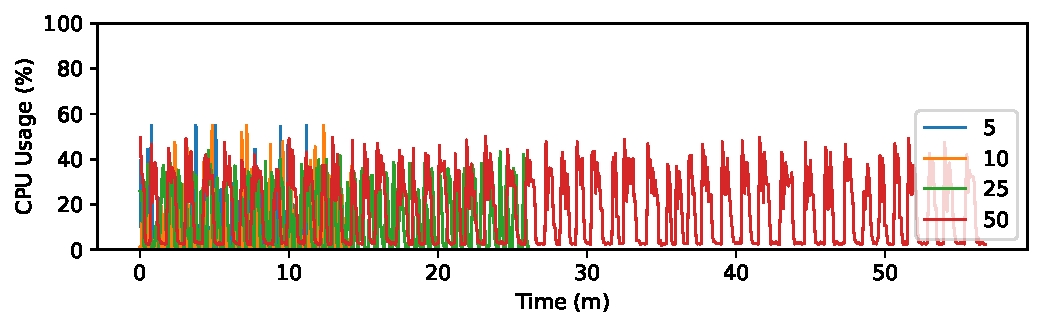
\includegraphics[width=\textwidth]{graphics/clients/cpu_multikrum_client.pdf}
        \caption{Multi-KRUM}
    \end{subfigure}
    \caption{CPU Usage on Training Clients Per Training Clients}
    \label{fig:cpu_clients_degree_clients}
\end{figure}

\begin{figure}[!h]
    \centering
    \begin{subfigure}[b]{0.49\textwidth}
        \centering
        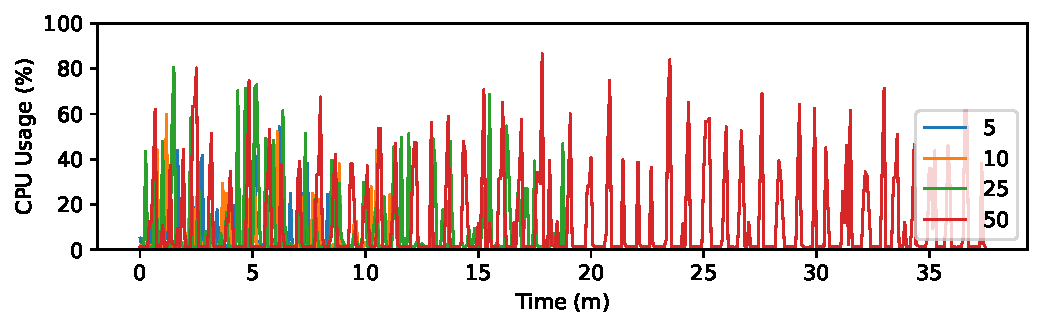
\includegraphics[width=\textwidth]{graphics/clients/cpu_none_server.pdf}
        \caption{None}
    \end{subfigure}
    \hfill
    \begin{subfigure}[b]{0.49\textwidth}
        \centering
        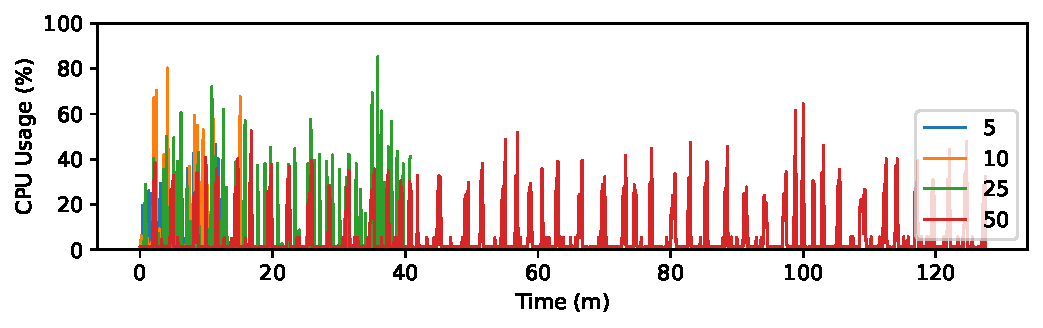
\includegraphics[width=\textwidth]{graphics/clients/cpu_blockflow_server.pdf}
        \caption{BlockFlow}
    \end{subfigure}
    \hfill
    \begin{subfigure}[b]{0.49\textwidth}
        \centering
        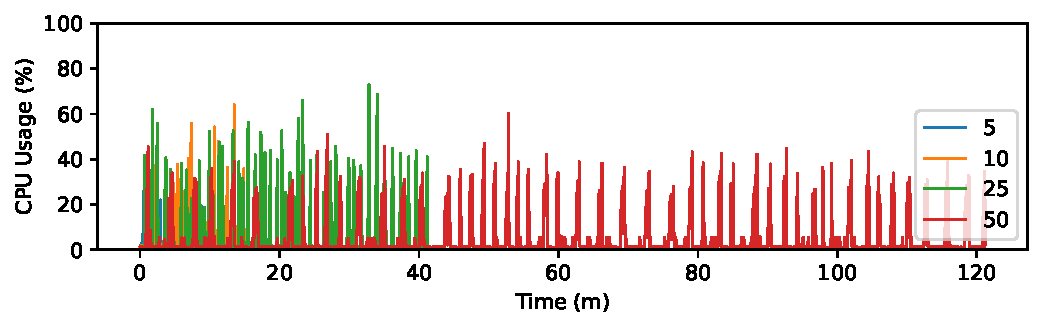
\includegraphics[width=\textwidth]{graphics/clients/cpu_marginalgain_server.pdf}
        \caption{Marginal Gain}
    \end{subfigure}
    \hfill
    \begin{subfigure}[b]{0.49\textwidth}
        \centering
        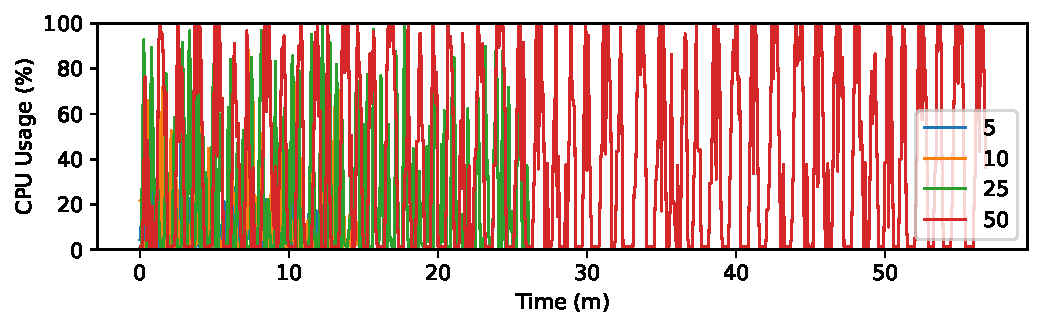
\includegraphics[width=\textwidth]{graphics/clients/cpu_multikrum_server.pdf}
        \caption{Multi-KRUM}
    \end{subfigure}
    \caption{CPU Usage on Computing Servers Per Training Clients}
    \label{fig:cpu_clients_degree_server}
\end{figure}

\begin{figure}[!h]
    \centering
    \begin{subfigure}[b]{0.49\textwidth}
        \centering
        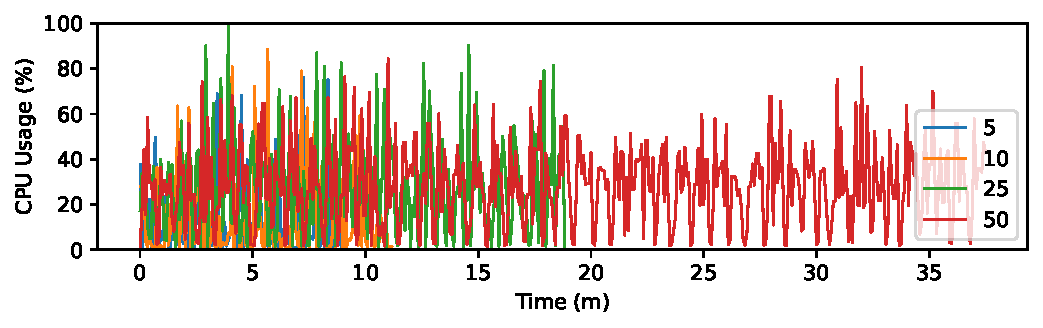
\includegraphics[width=\textwidth]{graphics/clients/cpu_none_miner.pdf}
        \caption{None}
    \end{subfigure}
    \hfill
    \begin{subfigure}[b]{0.49\textwidth}
        \centering
        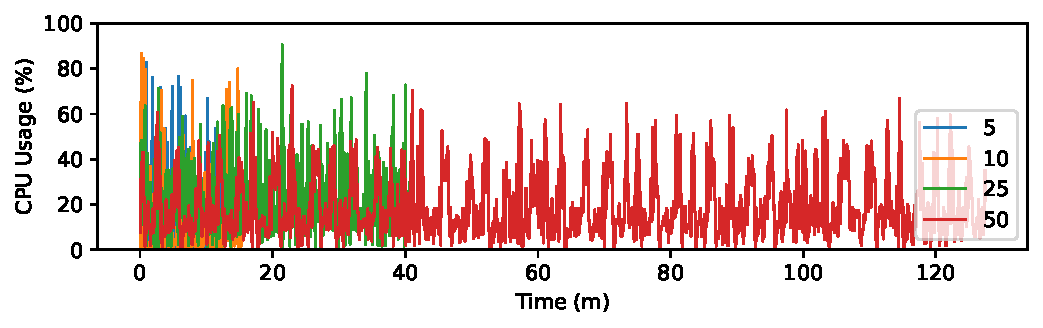
\includegraphics[width=\textwidth]{graphics/clients/cpu_blockflow_miner.pdf}
        \caption{BlockFlow}
    \end{subfigure}
    \hfill
    \begin{subfigure}[b]{0.49\textwidth}
        \centering
        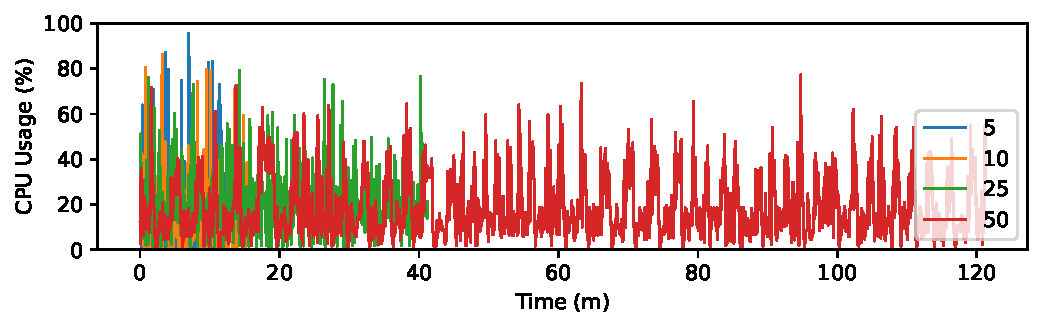
\includegraphics[width=\textwidth]{graphics/clients/cpu_marginalgain_miner.pdf}
        \caption{Marginal Gain}
    \end{subfigure}
    \hfill
    \begin{subfigure}[b]{0.49\textwidth}
        \centering
        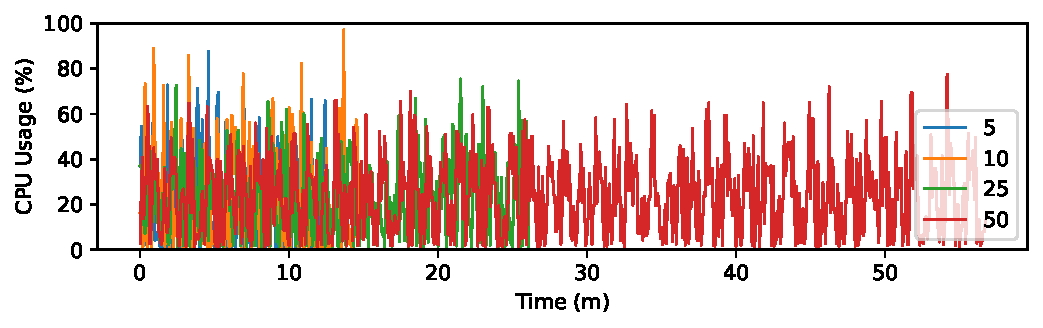
\includegraphics[width=\textwidth]{graphics/clients/cpu_multikrum_miner.pdf}
        \caption{Multi-KRUM}
    \end{subfigure}
    \caption{CPU Usage on Blockchain Nodes Per Training Clients}
    \label{fig:cpu_clients_degree_miner}
\end{figure}
